	\chapter{Object Detection}
	\label{sec:object_detection}
	
	On an abstract level the problem of object detection can be described by two individual tasks: Classification and Localization. While Classification deals with the question of what kind of object is displayed in the image, Localization is concerned with finding the position of objects. Hence, the output of a object detection system is usually a set of areas within the image and a corresponding class label. 
	
	Images are high dimensional signals that can contain a lot of information which is not relevant for the task. As the performance of most machine learning models decreases when the feature space becomes too large (curse of dimensionality), most computer vision pipelines can be separated in the stages of feature extraction, Classification/Localization. An overview is displayed in \autoref{fig:obj_pipeline}.
	
	\begin{figure}[hbtp]
	
	\centering
	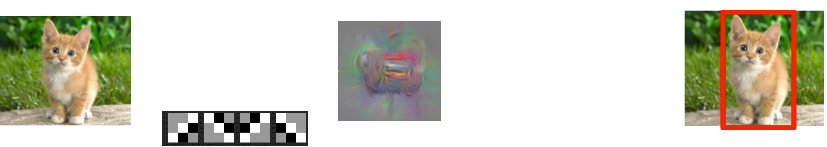
\includegraphics[width=\linewidth]{fig/ObjectDetection}
	\caption{Object Detection Pipeline.where $A_n$ describes an area, $C_1$ a class label, $I$ the image and $f$ the object detection function.}
	\label{fig:obj_pipeline}
	
	\end{figure}

	\begin{enumerate}
	\item The feature extraction stage extracts task relevant information from the image and infers an internal, more abstract representation. 
		
	\item The classification/localization stage produces the final output based on this representation. 
	
	\end{enumerate}  
	
	Commonly the areas $A$ are chosen as square bounding boxes. A lot of methods initially produce a lot of proposals that are fused to a final prediction with non-maximum suppression.
	
	Another way to reduce the input space, next to feature extraction, is the sampling method. While Sliding-window based techniques crop the image at different sizes and aspect ratios in top-left to bottom-right manner, Attention models try to employ a more targeted way of sampling. By focusing on the relevant parts of the image one tries to mimic the human vision process and to reduce the number of unnecessary computations. There are different ways to incorporate such an attention process into a detection pipeline. These will be further discussed \autoref{sec:object_detection:related}.
	
	In this thesis it is studied how a detection model can be applied to wire frame objects. Therefore a definition of wire frame objects is given. To the best of the authors knowledge the object class has not been previously defined or explicitly addressed by the research community.
	
	\paragraph{Definition - Wire Frame Objects}	\hfill \\
	The properties of wireframe object can be summarized in:
	\begin{enumerate}
		\item It does not consist of complex shapes but only basic geometric shapes like corners, edges
		\item The object parts themselves are thin structures.
		\item The object parts can be spread over large parts of the image.
		\item The object parts are sparse. The bounding box around the object is largely occupied by background
	\end{enumerate}
	
	The relevant research question of this chapter is stated as follows:
	
	\begin{center}
		\textbf{ How can a detection model represent wire frame objects?}
	\end{center}

	The question will be answered by doing a literature study and selecting several of the most promising methods for further experiments. The respective models are applied and evaluated in terms of performance. Furthermore, the insights of the models representation are studied.
	
	The rest of the chapter is organized as follows: \autoref{sec:object_detection:related} discusses relevant related work. Based on the gained insights \autoref{sec:object_detection:hypothesis} formulates several hypotheses to be investigated. \autoref{sec:object_detection:experiments} outlines the experiments conducted to evaluate the formulated hypotheses. \autoref{sec:object_detection:results} describes the obtained results. \autoref{sec:object_detection:conclusion} discusses the results and answers the research question.
	
	
	\section{Related Work}
	\label{sec:object_detection:related}
	The existing methods can broadly be grouped in three groups. Those are more traditional approaches without \acp{CNN}-based feature extraction, two-stage detectors and one-stage detectors.
	
	\section{Traditional Methods}
	
	"Traditional" is not a very precise term but has also been used in other publications to  group methods that don't use the recently very popular \acp{CNN}-feature extractor. Therefore the term is similarly used in this work.
	
	One of the first object detection methods was \cite{Viola2004} that used simple filters inspired by Haar-basis functions as a feature extractor for human face detection. The image was processed in a cascade of classifiers that assigned the label "face" or "background" to image patches. The output of the first stages were further classified when going deeper in the cascade. To employ an attention process, the processing of one image patch stopped, when a classifier assigned the label "background".
	
	Although being very fast the Haar-based feature extraction was not very robust towards rotation-, scale- or shape-variations \todo{quote}. A more robust feature extractor was proposed by \cite{Dalal} and \cite{Lowe2004} for pedestrian detection. A local (normalized) histogram of gradients is computed for a fixed window size. 

	However, these methods prove to be sensitive towards part occlusions or large deformations. This gave raise to deformable part models where parts of the object are explicitly learned and detected.  \todo{describe springs}

	
	Guido proposes a neural network to learn an attention model.
	
	X propose a recurrent neural network architecture to model the attention process.
	
	\section{\acp{CNN}-based Detectors}
	
	In recent years \acp{CNN} emerged from deep learning research and became a popular feature extractor. \acp{CNN} can be seen as small neural networks that are applied locally on image patches at various locations. In contrast to manually designed methods, \acp{CNN} can be learned task specific via back-propagation.
	
	With $i,j$ as location, $y$ as output, $f$ as activation function, $W$ as filter weights, $X$ as input and $b$ as bias, the convolution operation can be expressed as follows:
	
	$$Y_{ij} = f(WX_{ij} + b)$$
	
	where the size of $W$ depends on the kernel size $k$ and the locations are usually chosen in sliding window manner with a certain step size $s$, also called strides.
	
	\acp{CNN} offer the advantage that they can be stacked on top of each other and therefore be combined in several layers to learn highly non-linear representations.
	\todoref{arg1} demonstrate a very efficient architecture in which only 3x3 kernels are used. That way early layers focus on fine grain details and basic features like edges and corners, while higher order layers combine these features to more complex shapes. 
	
	Various studies suggest that going deeper with convolutions increases representation strength yielding even better results. However, such high performance comes at a cost. As \acp{CNN} grow deeper inference time and memory usage increase as well.
	
	Next to the standard convolutional kernel several variations can be found in literature: Atrous/Dilated convolutions consist of a sparse kernel thereby increasing the receptive field of a filter without increasing complexity or number of computations \todoref{Atrous}. Deformable convolutions allow a kernel shape different from the standard symmetric kernel \todo{deformable cnn}.
	
	Different activation functions have emerged. $Tanh$ and sigmoid-activations produce naturally an output at a small range which simplifies the optimization. However, when the filter output falls unfavourably, the gradient with respect to the activation is almost zero leading to much longer training times. This issue gave rise to the family of rectified linear units (ReLU) which have been generalized in \todoref{..} to parametrized linear units (PReLU):
	
	$$
	f(x) = \begin{cases}
	x \quad \text{for } x \geq 0 \\
	\alpha x \quad \text{for } x < 0
	\end{cases}
	$$
	
	The issue of network initialization and "saturating" activations is also addressed in \cite{Ioffe2015}. With batch normalization the authors introduce a layer that normalises the data batch-wise and is fully differentiable. Including batch normalization after a convolutional layer leads to more stable and faster convergence. \todoref{arg1} show how using batch normalization cancels out the bias term.
	
	Using a convolutional layer followed by batch normalization and non-linear activation evolved to a standard in classification and object detection pipelines. It can be summarized in:
	
	\todo{doublecheck}
	$$
	Y_{ij} = f(\frac{WX_{ij}}{\sigma}+c)
	$$
	
	\todo{Residual Connections}
	
	
	\todo{other architectural stuff}
	
	
	Various authors show how \acp{CNN}-based methods outperform methods with engineered feature extractors by far\todoref{Alexnet,}. \cite{Razavian}s experiments show how that this is not only because \acp{CNN}-features are trained on a specific task, but that  the learned representation is quite general and can be used in other vision tasks and methods.
	
	This has led to common practice to train feature extractors with a classification task on the Imagenet dataset with \todo{number} images and to use these weights to initialize networks for other tasks like object detection or segmentation. Popular feature extractors are summarized in \autoref{tab:cnn-extractors}.
	
	\begin{table}[htbp]
		\centering
		\caption{Popular Feature Extractors}
		\begin{tabular}{l|l|l|l}
			Name & Layers & Number of Weights &  \\ \hline
			VGGNet &  &  &  \\ \hline
			ResNet &  &  &  \\ \hline
			GoogLeNet &  &  &  \\ \hline
			MobilenetV2 &  &  &
		\end{tabular}
		\label{tab:cnn-extractors}
	\end{table}

	After the performance boost for image classification \acp{CNN} have also been employed for the task of object detection. The existing methods can be grouped in two apporaches.
	
	
	\subsection{Two-stage Approaches}
	
	Two-stage approaches consists of a first stage that proposes regions, likely to contain an object and second stage that classifies these objects. In a way the first stage models an attention process such that the second stage can focus on the relevant parts of the image.
	
	The first method to employ a two stage approach was R-CNN that used the Selective Search algorithm\todoref{sel. search} for region proposal and \acp{CNN}-based classifier for the second stage. As the second stage was an expensive method that had to be run at various scales and regions of the input image, the approach was computationally intense while containing a lot of redundant operations. In the following years research was conducted to combine more steps of the approach to save computations. Fast-RCNN \cite{Ren} used a \acp{CNN} to generate the region proposals while using an SVM classifier for the second stage. Faster-RCNN \cite{Ren2015} proposes a fully \acp{CNN}-based pipeline that can be trained end-to-end on the task of object detection.
	
	
	\subsection{One-stage Approaches}
	
		\iffalse
	\begin{figure}[hbtp]
		
		\centering
		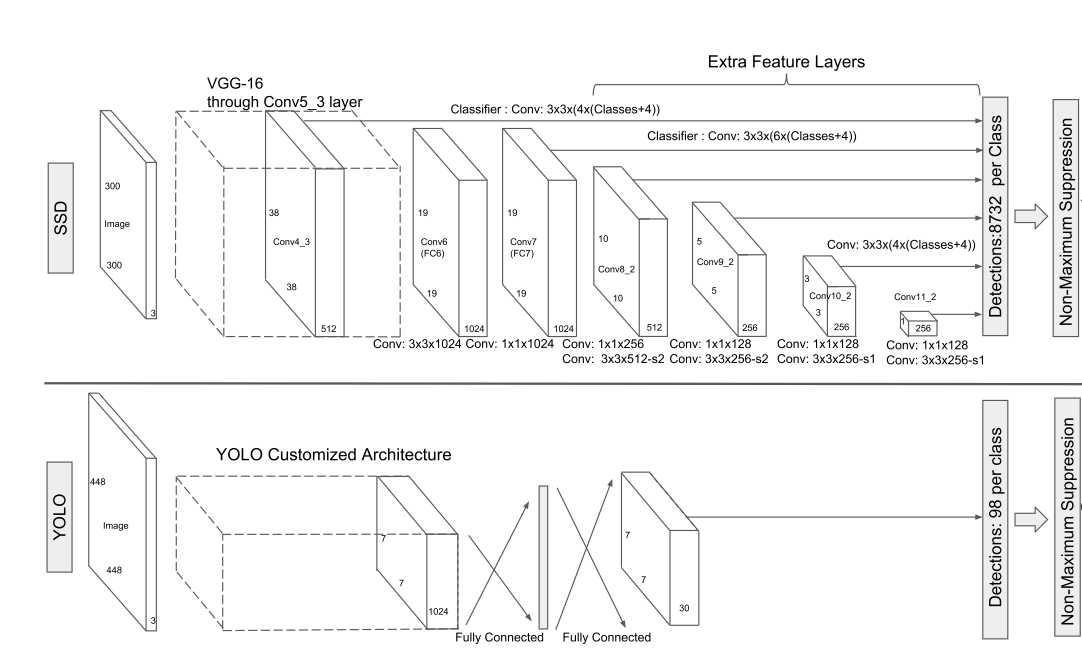
\includegraphics[width=\linewidth]{fig/architecture}
		\caption{Typical Architecture for One Stage Detectors}
		\label{fig:architecture}
		
	\end{figure}
	\fi
	Regression models incorporate all stages of object detection in one model and formulate the task as regression problem. Predictions are made for a predefined set of regions. The process is usually modelled with deep neural networks.
	
	\citeauthor{Redmon} were the first to publish such a method in \cite{Redmon}. The task is formulated by dividing the input image in a fixed grid and defining output nodes with softmax activation to predict $C$ class probabilities for each grid cell. Additional $5*B$ output nodes predict $B$ set of bounding box coordinates and $B$ object probabilities for each cell. This leads to a total number of $S*S*B*(4 + 1 + C)$ output nodes. 
	
	YoloV2, SSD  formulate the task by discretizing the output as a set of preparameterized bounding boxes. For each box class probabilities and bounding box offsets are predicted. In total this leads to $S*S*B*(4 + 1 + C)$ output nodes. 
	
	The models are trained by assigning a certain set of output nodes the "responsibility" to predict a certain object. That means only the output for these nodes is taken into account when calculating the loss for a certain sample and when updating the weights in the backward pass. This "matching strategy" is usually based on the intersection-over-union between ground truth and anchor box. \autoref{fig:anchors} illustrates the concept in the example of SSD.  
	
	\begin{figure}[hbtp]
		
		\centering
		\captionsetup{justification=raggedright,singlelinecheck=false}
		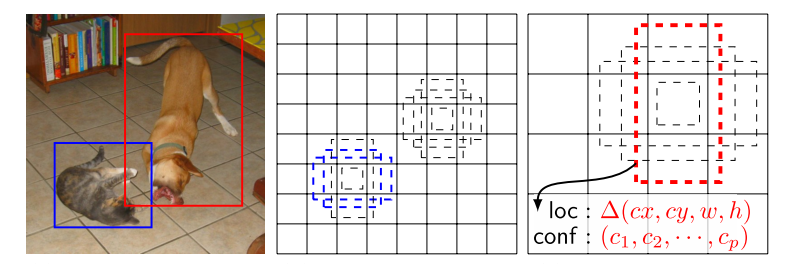
\includegraphics[width=0.8\linewidth]{fig/anchors}
		\caption{The anchor boxes are displayed as dashed lines. The ground truth label of the cat in blue is assigned to two anchor boxes. The output nodes predicting coordinate offset $\Delta(cx, cy, w,h)$ and class probabilities $c_1 .. c_p$ corresponding to these two boxes take part in the loss calculation \cite{Liu}.}
		\label{fig:anchors}
		
	\end{figure}
	
	Within this framework several approaches exist that either change the base network or modify layers in between: \cite{ChengchengNing2017} propose propose a more efficient non-max-suppression method as well as to include an inception module in the network architecture to reduce computation while keeping/increasing performance. \cite{Wu} uses \textit{SqueezeNet} as base network and a mixture between the ssd and yolo loss function as training goal. \cite{Xiang} investigates the receptive fields of SSD and tries to incorporate more context, especially on lower feature maps, to increase detection rate for small objects.\cite{Linb} applies the framework for vehicle detection. They use \textit{GoogLeNet} as base network (and investigate several others).\cite{TripathiSanDiego} apply a network very similar to YoloV2 and investigate 8bit quantization of the model to make it runnable on embedded devices.
	
	A common problem of one stage detectors is the imbalance between background and object samples. Most methods upweigh the positive samples and/or use hard negative mining. \cite{Lin} introduces the \textit{Focal Loss} which focuses on sparse positive samples by design.
	
	Each of the described group of methods has strengths and weaknesses. While shallow methods are typically quite fast they require a lot of manual effort and/or are not so accurate. Two-stage detectors on the other hand are quite accurate but their computational requirements are prohibitive for the hardware to be used in this thesis. One-stage detectors offer a compromise between detection accuracy and inference speed. In addition they can be trained end-to-end which requires only little manual engineering. However, the presented methods are still too slow for the hardware used in this thesis.


	

	%			\paragraph{Scalable Object Detection using Deep Neural Networks\cite{Erhan}}
	%			\begin{itemize}
	%				\item[-] Generates number of bounding boxes as object candidates (class agnostic) and confidences for each box
	%				\item[-] For each Bounding Box a classifier is run e.g. DNN
	%				\item[-] Training: If the number of boxes k is larger than the number of objects b, only b boxes are matched while the confidence of the others is minimized
	%				\item[-] Assignment problem $$F_{match}(x,l) = \frac{1}{2}\sum_{i,j}x_{ij}||l_i - g_j||^2_2$$ where $x_ij$ is one if the ith prediction is assigned to the jth ground truth object
	%				\item[-] Confidence: 
	%				$$F_{conf}(x,c) = - \sum_{i,j}x_{ij}*\log(c_i)-\sum_{i}(1-\sum_{j}x_{ij})\log{1-c_j}$$
	%				\item[-] Speed up training by clustering (kmeans) of ground truth and using it as prior (prior matching)
	%				\item[-] Can be defined to output boxes only for a particular class by training the bounding boxes on that class
	%				\item[-] Number of parameters grows linearly with number of classes
	%				\item[-] Authors argue two step process (region proposal + classification) is better
	%				\item[-] Architecture based on AlexNet
	%				\item[-] Predicted boxes are merged using non-maxima surpression
	%				\item[-] One shot(50\%), +2scales (75\%)
	%				\item[-] OverFeat/ Selective Search are faster but much more expensive
	%			\end{itemize}
	



\section{Wire-frame objects}

\todo{Definition of a wireframe object}


\todoref{Wire detection}
\todoref{Method from last year, Other papers on drone racing}

\todo{Compare the individual methods, based on the literature and previous results formulate a hypothesis}

\section{Hypothesis}

Several hypothesis are formulated and will be examined experimentally:
\begin{enumerate}
	\item \textbf{A \acp{CNN} should be able to learn the object detection task.}
	\item \textbf{For wireframe objects the deeper layers don't learn anything as the object consist of relatively simple shapes.}
	\item \textbf{The detection of fine grain structures is important.}
\end{enumerate}
\newpage
\section{Experiments}

First we show that many weights in an object detector are superflous when detecting single wire frame objects:
1. We train an object detector on a single but complex object and compare the filters to multiple objects
2. We train an object detector on a single wireframe object and compare the filters to the other feature detectors
3. We use the gained insights to prune the network 
4. The pruned network should perform poorly when used on the complex object
4. We analyse the new network in terms of sensitivity towards: occlusion, colour, distance, angle

\section{Results}

\section{Conclusion}